\documentclass[11pt]{article}
\usepackage{graphicx}
\marginparwidth 0pt
\oddsidemargin  0pt
\evensidemargin  0pt
\marginparsep 0pt
\usepackage{amsmath}
\topmargin 0pt
\usepackage{mathtools}
\textwidth   6.5 in
 \textheight  8 in
\usepackage{fancyhdr}
\renewcommand{\headrulewidth}{2pt}
\renewcommand{\footrulewidth}{1pt}
 
\pagestyle{fancy}
\usepackage{amsmath}
 %%%%%%% %%%%%%% %%%%%%% %%%%%%% %%%%%%% %%%%%%%For python%%%
 % Default fixed font does not support bold face
\DeclareFixedFont{\ttb}{T1}{txtt}{bx}{n}{12} % for bold
\DeclareFixedFont{\ttm}{T1}{txtt}{m}{n}{12}  % for normal

% Custom colors
\usepackage{color}
\definecolor{deepblue}{rgb}{0,0,0.5}
\definecolor{deepred}{rgb}{0.6,0,0}
\definecolor{deepgreen}{rgb}{0,0.5,0}

\usepackage{listings}



% Python style for highlighting
\newcommand\pythonstyle{\lstset{
language=Python,
breaklines=true,
basicstyle=\ttm,
otherkeywords={self},             % Add keywords here
keywordstyle=\ttb\color{deepblue},
emph={MyClass,__init__},          % Custom highlighting
emphstyle=\ttb\color{deepred},    % Custom highlighting style
stringstyle=\color{deepgreen},
frame=tb,                         % Any extra options here
showstringspaces=false            % 
}}

%++++++Hyperlink
\usepackage{hyperref}
\hypersetup{
    colorlinks=true,
    linkcolor=blue,
    filecolor=magenta,      
    urlcolor=cyan,
}

%%For table
\usepackage{array}
\newcolumntype{L}[1]{>{\raggedright\let\newline\\\arraybackslash\hspace{0pt}}m{#1}}
\newcolumntype{C}[1]{>{\centering\let\newline\\\arraybackslash\hspace{0pt}}m{#1}}
\newcolumntype{R}[1]{>{\raggedleft\let\newline\\\arraybackslash\hspace{0pt}}m{#1}}




% Python environment
\lstnewenvironment{python}[1][]
{
\pythonstyle
\lstset{#1}
}
{}

% Python for external files
\newcommand\pythonexternal[2][]{{
\pythonstyle
\lstinputlisting[#1]{#2}}}

% Python for inline
\newcommand\pythoninline[1]{{\pythonstyle\lstinline!#1!}}
%%%%%%%%%%%%%%%%%%%%%%%%%%%%%%%% %%%%%%% %%%%%%% %%%%%%%


%\pagestyle{empty}

\begin{document}


\begin{center}
  {\bf
  CS 534 Machine Learning  }

\vspace{12pt}

  Project 3, due Sunday, April 15
  \\
  Chenxi Cai \\
  Yifei Ren \\
  Qingfeng (Kee) Wang
 
\end{center}

\vspace{12pt}




\clearpage
(Notice, all links (table of contents, figures references, table references etc.) are clickable! You can download this PDF and open it using Preview or Adobe Reader to enable this convenient feature.)
 
\tableofcontents{}

\clearpage


\section{Introduction and methods}
Convolutional neural network (CNN) proves to be one of the most successful training models. This time we will use CNN to train MNIST data which is a database of handwritten figures in black and white. It contains 55000 training images and 10000 testing images. In this report, we will split 55000 training data into 80\% data for training and 20\% for validation. All data are trained in 5000 steps. Validation data accuracy and loss were monitor in every 500 steps. Gradient were calculated in batch size 200.


We constructed a base model and then adjust  hyper-parameters in two stages. 

First, in section \ref{stage1}, we tune the size and number of the filters, number of convolution and polling layers, learning rate, the ways of paddings and the choices of activations functions. After choosing the optimized hyper-parameters, we finally the behavior of three different optimizers in section \ref{stage2}. 

A more detailed discussion of finally chosen model is provided in the section \ref{summary}. At the end of the report, code of base model is provided.



\section{Adjust hyper-parameters: stage I}
\label{stage1}
In this section we first adjust several hyper-parameters listed in the requirement 2. Hyper-parameters are determined by the validation accuracy (or loss) and the time efficiency.


\subsection{Size of the filters}
In base model, the size of filter is 5-by-5. According to Stanford University video courses lecture 5, common settings of filter size are listed in the Table \ref{tab:fsp}.


\begin{table}[!htb]
\centering
\caption{Commonly adjusted filter sizes. Where F is filters' spatial extend (filter dimension), S is the stride, P is the amount of zero padding. 
}
\label{tab:fsp}
\begin{tabular}{C{3cm} C{3cm} C{3cm}}
\hline \hline

F	&S	&P		 \\ \hline 
3	&1	&1 \\
5	&1	&2 \\
1	&1	&0 \\ \hline \hline

\end{tabular}
\end{table}

Here we tried three different cases of filter's size: $1\times1$, $3\times3$ and $5\times5$. 

Now we know that the final accuracy after 5000 steps are shown in Table \ref{tab:filter}. From the table we can obtain that $5\times5$ is the best size.

\begin{table}[!htb]
\centering
\caption{Validation accuracy at 5000 steps }
\label{tab:filter}
\begin{tabular}{C{5cm} C{2cm} C{2cm} C{2cm}}
\hline \hline

Size of filters	&$1\times1$	&$3\times3$	&$5\times5$		 \\ \hline  
Accuracy	&0.7676	&0.9133	&0.9252 \\ \hline \hline

\end{tabular}
\end{table}



\subsection{Number of filters}
In base model, filter number is 32 for conv 1 and 64 for conv 2. According to Stanford University video courses lecture 5, common settings of filter number are power of 2: 32, 64, 128 and 512, etc.

Here we tried four different combinations of number of filters (conv1, conv2): (32, 32), (32, 64), (64, 64) and (128, 128). Now we know that the final validation accuracy at 5000 steps are shown in Table  \ref{tab:num-filter}.

\begin{table}[!htb]
\centering
\caption{Validation ccuracy at 5000 steps}
\label{tab:num-filter}
\begin{tabular}{C{6cm} C{2cm} C{2cm} C{2cm} C{2cm}}
\hline \hline

Number of filter (conv1, conv2)	&(32, 32)	&(32, 64)	&(64, 64)	&(128, 128)		 \\ \hline
Accuracy at 1000 step  	&0.5977	&0.7482	&0.7333	&0.7294 \\
Accuracy at 5000 step	&0.9221	&0.9275	&0.9268	&0.9265 \\ \hline \hline
\end{tabular}
\end{table}


From the table, the accuracy increases little with number, the final accuracies are very close. However, from the accuracy plots, we ca see that the initial accuracies at 1000 steps have large differences. In according to the loss trending shown Figure \ref{fig:filter_number}, all four models shows similar loss descending curves with filter (32, 64) the steepest. It also should be noted filter size greater than (32, 64) takes a lot more time to finish the training but only gives marginal accuracy improvement. As a result, it is easy to conclude that filter (32, 64) is the best choice. 

\begin{figure}[!htb]
   \centering
   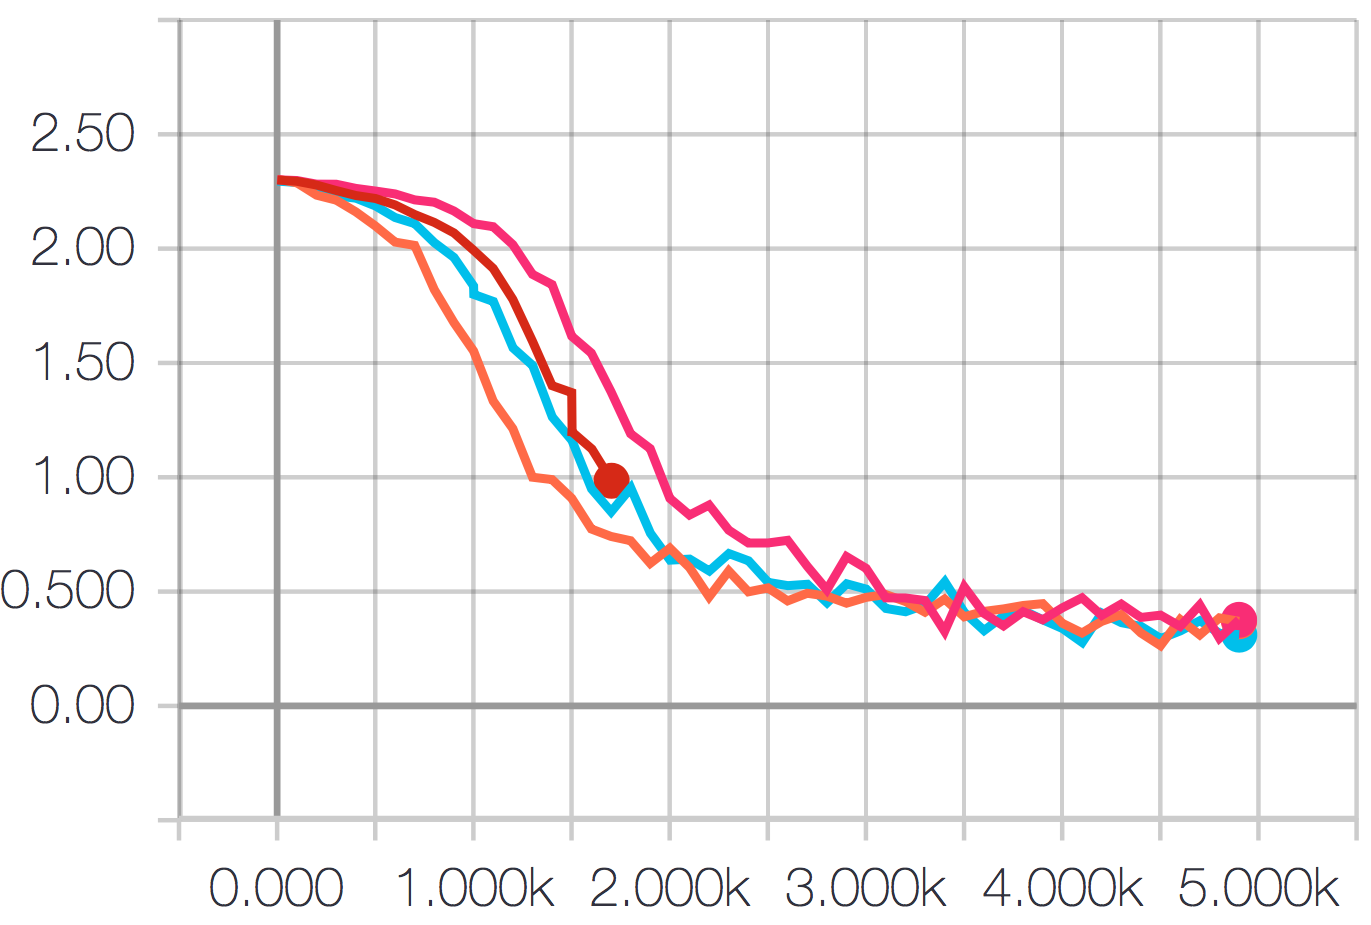
\includegraphics[width=10cm]{images/filter_number.png} % requires the graphicx package
   \caption{The figure shows the trend of loss function behavior of different filters. The steepest curve at bottom belongs to filter (32, 64). See tensorboard event file for detailed legend.}
   \label{fig:filter_number}
\end{figure}


\clearpage
\subsection{Number of convolution and pooling layers}
This is somewhat harder to tune. Generally, we have one pooling layer after a convolutional layer, and the dimension is cut into half. Begin with single image size $28\times 28$, it is easy to see we can apply at most 2 pooling layers if we are using {\tt same} padding. As a result, we only choose 1 convolutional layer plus 1 pooling layers (structure shown in Figure \ref{fig:1-c-1-p}) and 2 convolutional layers plus 2 pooling layers (base model,  structure shown in Figure \ref{fig:2-c-2-p}) ) to compare.

The behavior of two different CNN structures are shown in Figure \ref{fig:structure}. At 5000 step, the base model have a lower loss. As a result, we choose 2 convolutional layers plus 2 pooling layers as the final structure.


\begin{figure}[!htb]
   \centering
   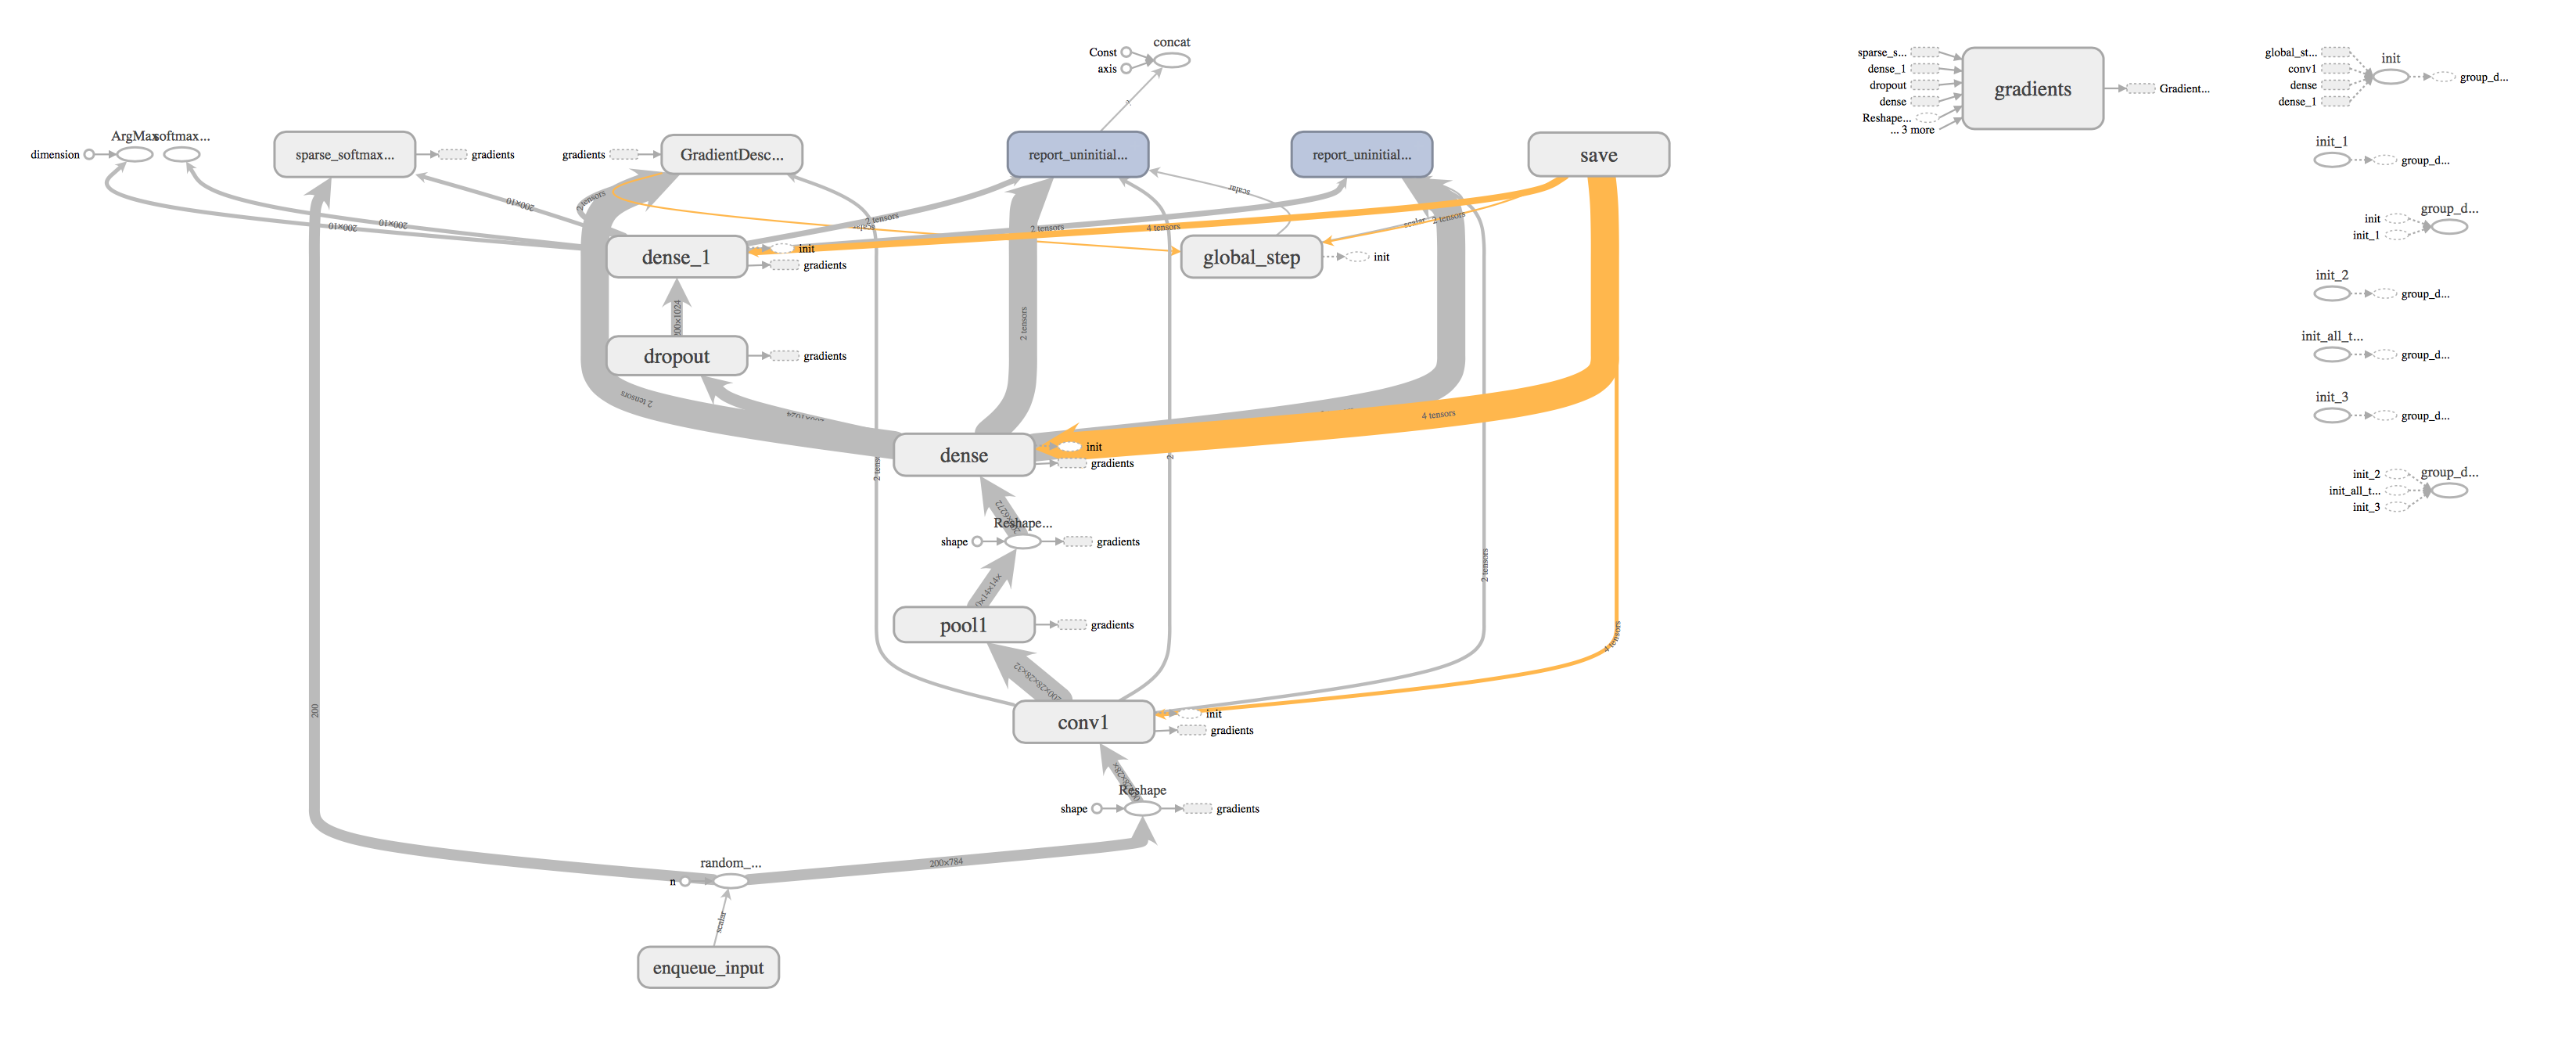
\includegraphics[width=16cm]{images/graph-conv1-pool1.png} % requires the graphicx package
   \caption{Graph for 1 convolutional layer and 1 pooling layer. Zoom in to see details.}
   \label{fig:1-c-1-p}
\end{figure}


\begin{figure}[!htb]
   \centering
   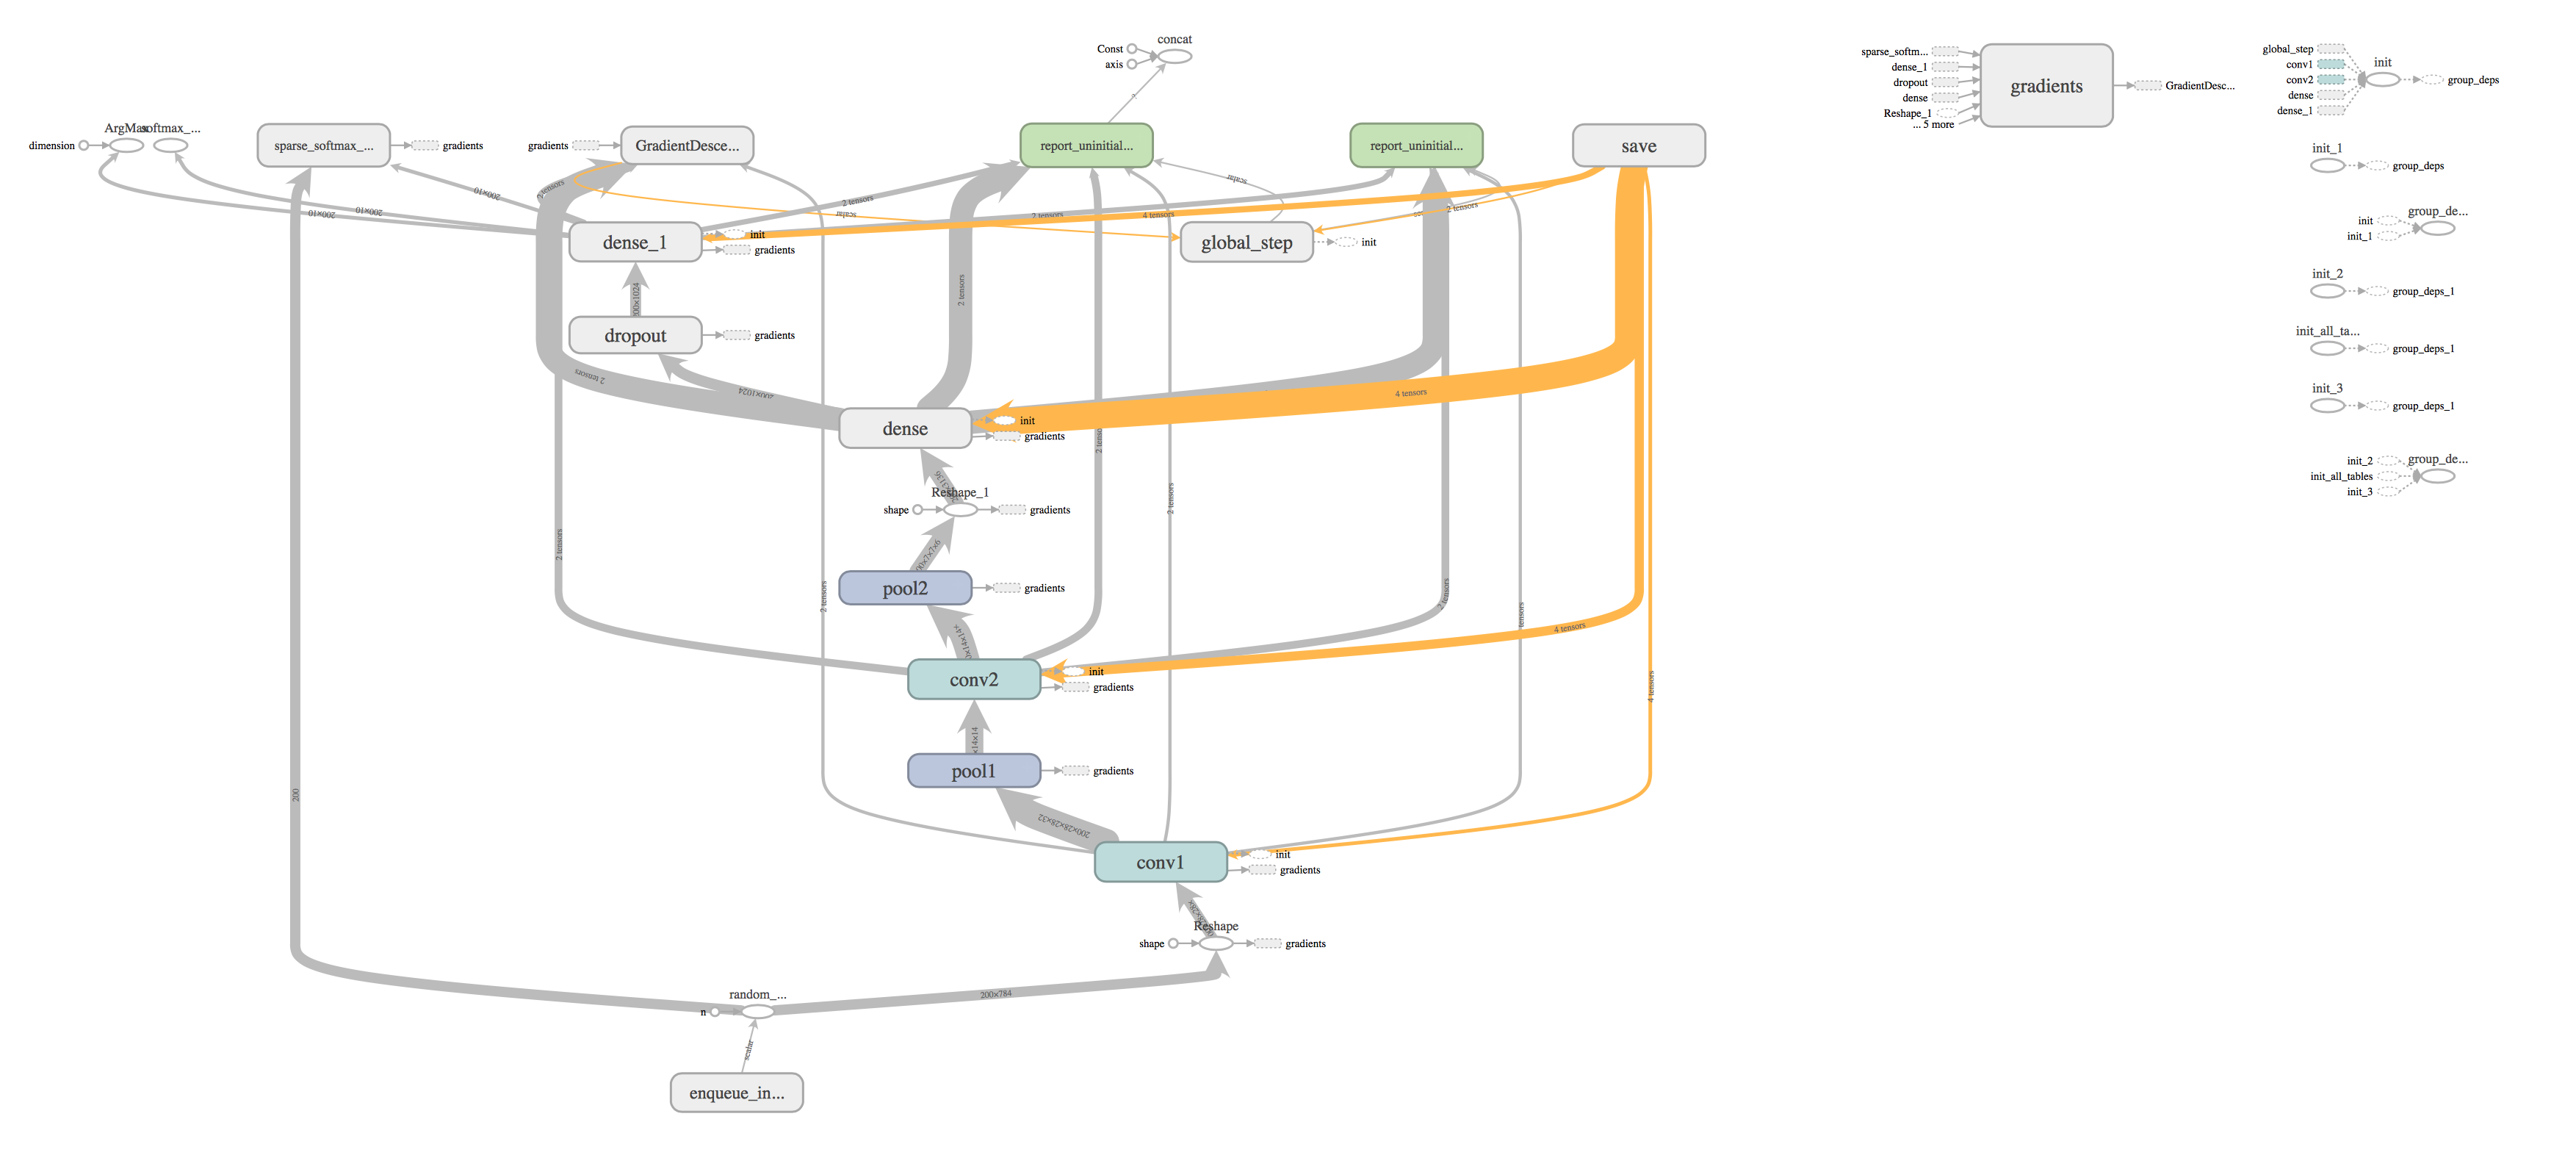
\includegraphics[width=16cm]{images/graph-conv2-pool2.png} % requires the graphicx package
   \caption{Graph for 2 convolutional layers and 2 pooling layer.Zoom in to see details.}
   \label{fig:2-c-2-p}
\end{figure}

\begin{figure}[!htb]
   \centering
   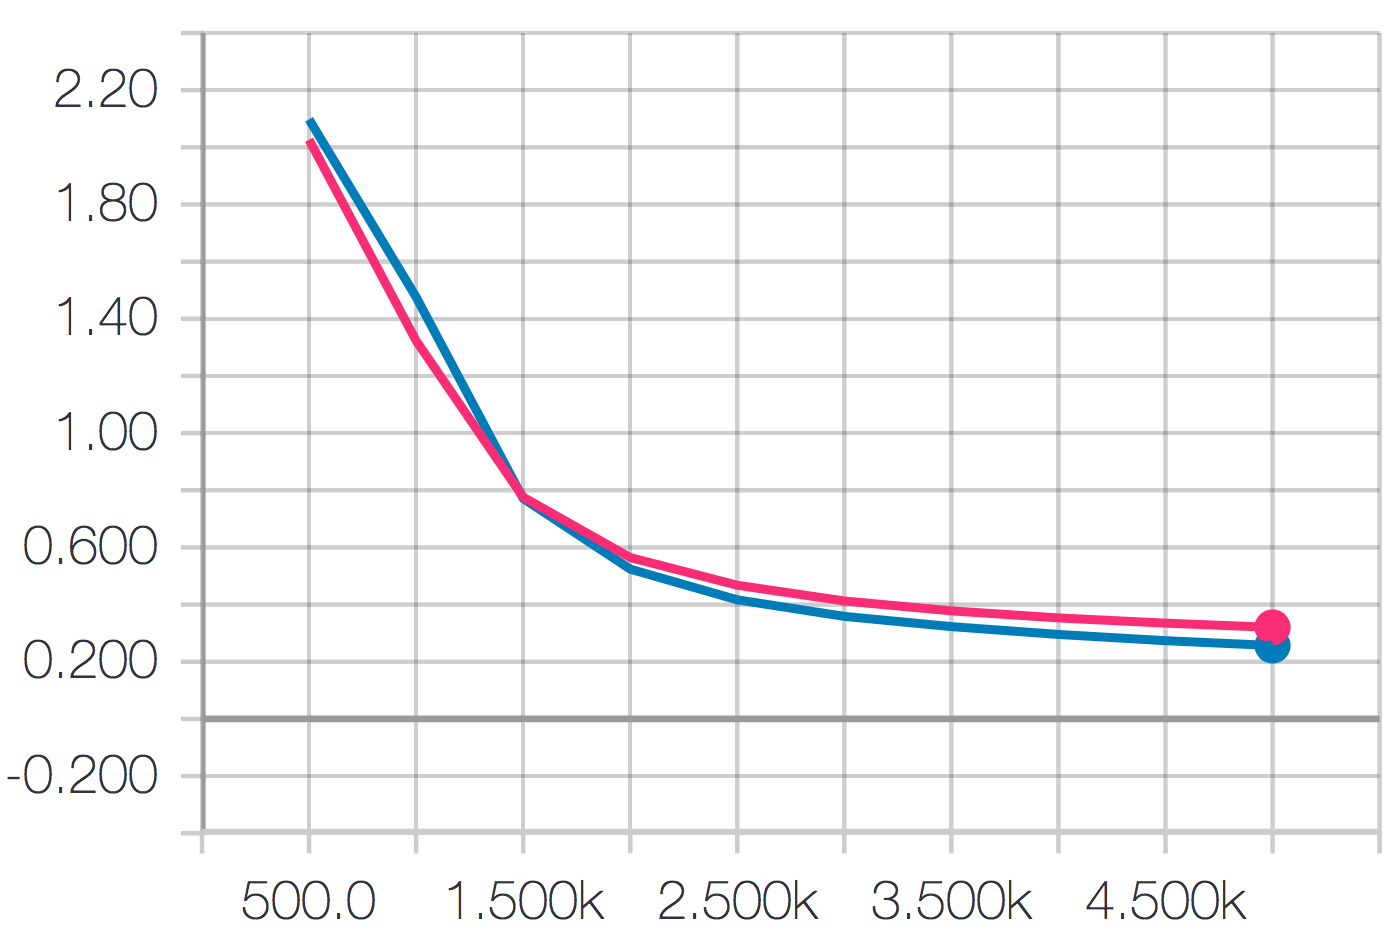
\includegraphics[width=10cm]{images/structure.png} % requires the graphicx package
   \caption{The comparison of loss of two different CNN structures. Red curve, with final loss 0.3203, correspond to 1 convolutional layer and 1 pooling layer. Blue curve, with final loss 0.2567, correspond to 2 convolutional layers and 2 pooling layers.}
   \label{fig:structure}
\end{figure}

\clearpage

\subsection{Learning rate}
There are several choices of learning rate from {\tt 1E-5, 1E-4, 1E-3, 1E-2, 1E-1} to {\tt 1}. It seems the best learning rate is {\tt 1E-1} as it converges to a very high accuracy (low loss) very fast. The Figure \ref{fig:lr} shows the trend of learning rate. The loss of curve steadily decrease faster as we increase learning rate from {\tt 1E-5} to {\tt 1E-1}. However, when learning rate equals to {\tt 1}, the loss function remains around 2.25 and does not decrease. As a result, learning rate at {\tt 1E-1} is the the best learning rate we choose.




\begin{figure}[!htb]
   \centering
   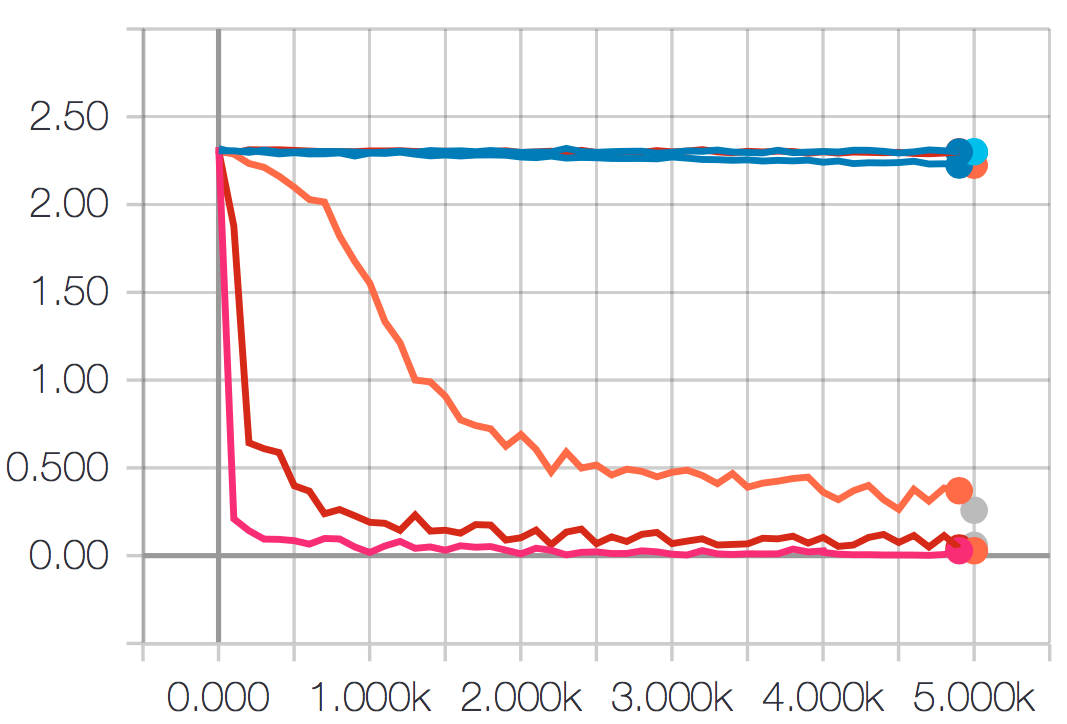
\includegraphics[width=10cm]{images/learning_rate.png} % requires the graphicx package
   \caption{Loss function of training data. The detailed assignment of curves is shown in the event file and can be viewed in Tensorboard. The curve that descent the fastest correspond to learning rate equals to {\tt 1E-1}.}
   \label{fig:lr}
\end{figure}




\clearpage
\subsection{The ways of paddings}
So far there are two types of padding methods, i.e., {\tt same} (base model) and {\tt valid}. Here we compared the difference between {\tt same} and {\tt valid}. The accuracy is presented in Figure \ref{fig:padding}. It is obvious that using {\tt same} padding always gives the better accuracy in this test case. The loss of training is presented in Figure. \ref{fig:padding_loss} and shows that the loss of training data decreases much faster when using {\tt same} padding. It can be inferred that {\tt same} padding gives the best result and is the final hyper-parameter we chose.


\begin{figure}[!htb]
   \centering
   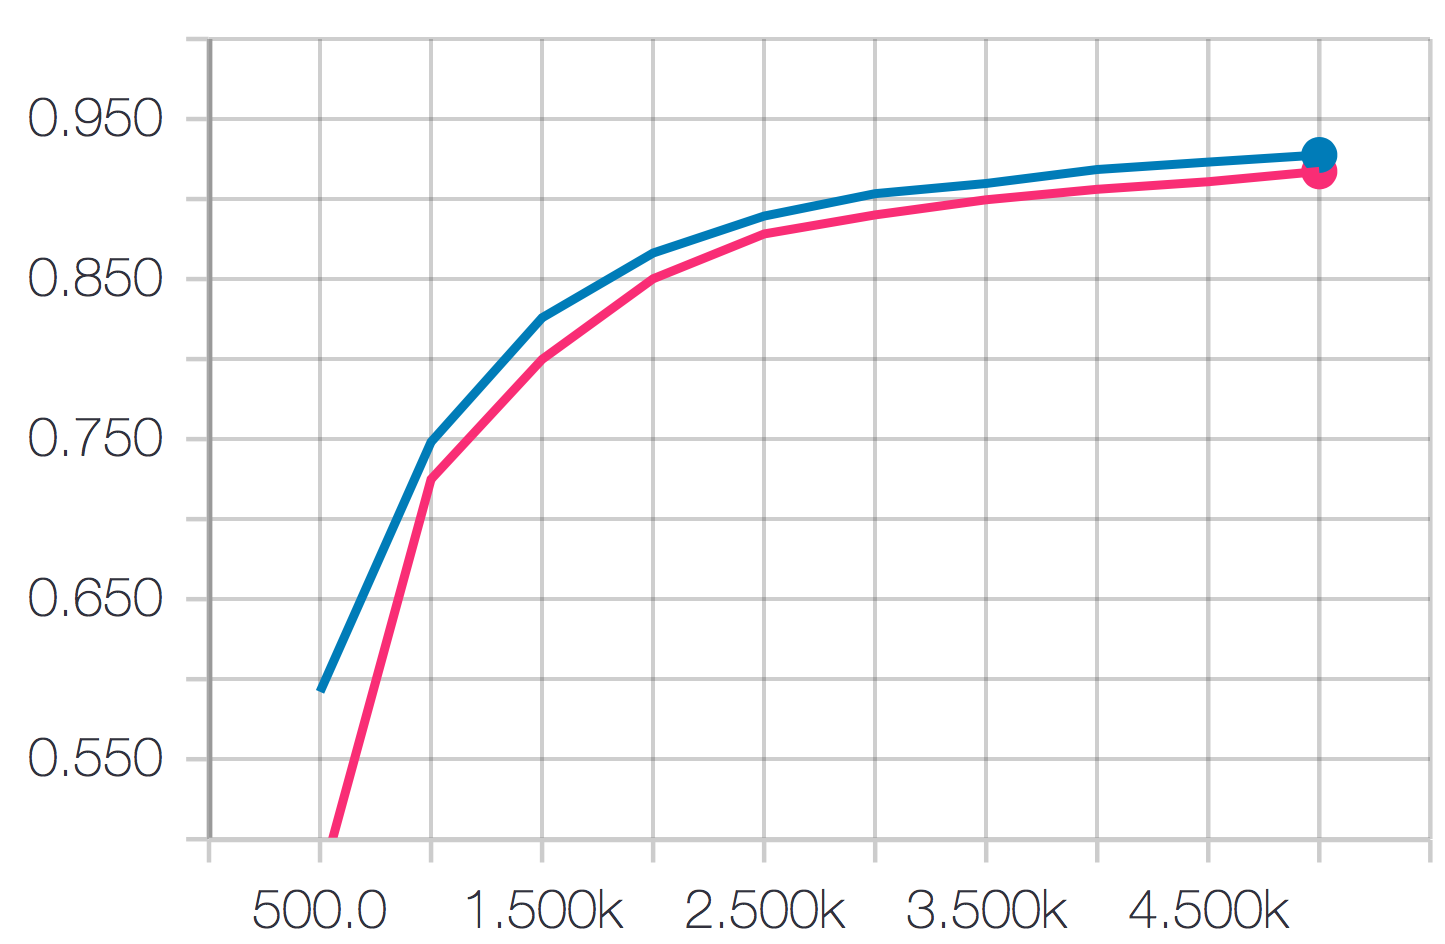
\includegraphics[width=8cm]{images/padding_accuracy.png} % requires the graphicx package
   \caption{The figure shows the accuracy of validation data of {\tt same} (blue) and {\tt valid} (magenta) padding. }
   \label{fig:padding}
\end{figure}



\begin{figure}[!htb]
   \centering
   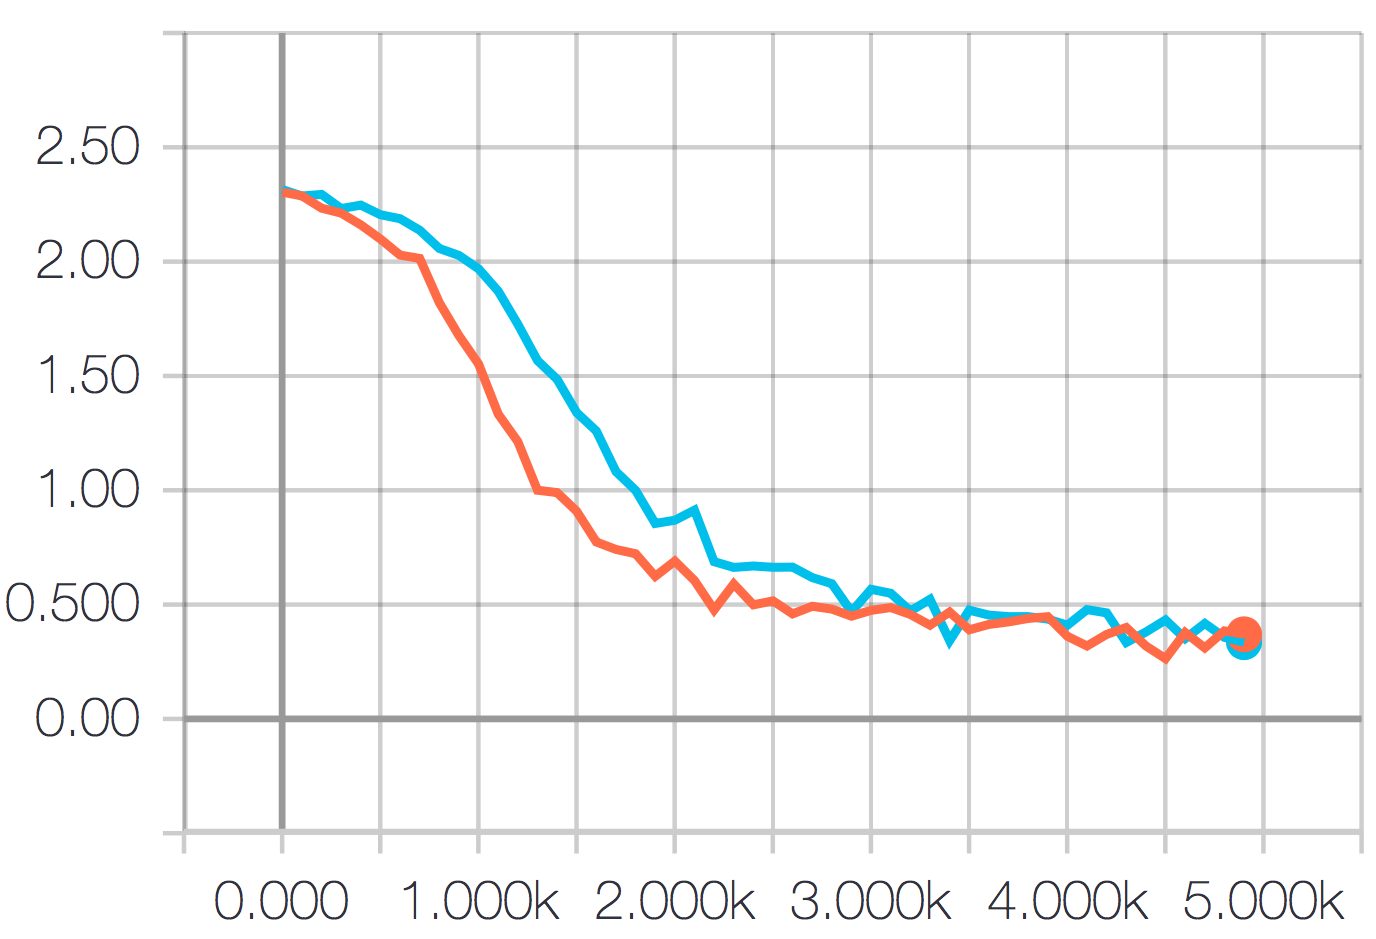
\includegraphics[width=8cm]{images/padding_loss.png} % requires the graphicx package
   \caption{The figure shows the loss training data of {\tt same} (orange) and {\tt valid} (cyan) padding. }
   \label{fig:padding_loss}
\end{figure}



\clearpage

\subsection{The choices of activation functions}
(To be finished by Yifei)
The training loss is shown in Figure \ref{fig:af_loss} while the validation accuracy is shown in Figure \ref{fig:af_accuracy}. Obviously Sigmoid activation function does not learn much in this test case. As a result we chose {\tt ReLu} as our final hyper-parameter.


\begin{figure}[!htb]
   \centering
   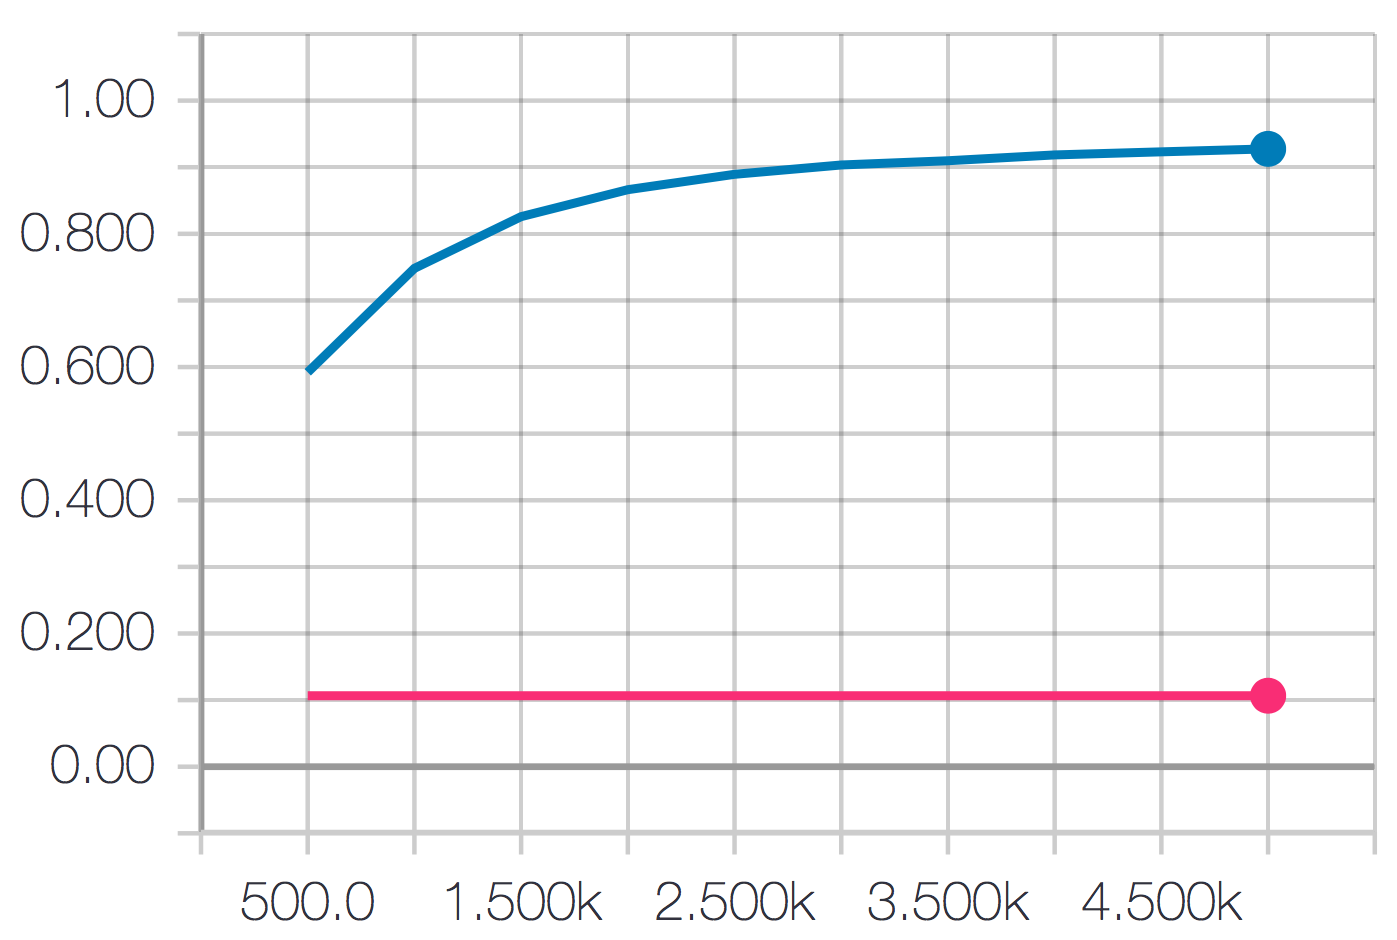
\includegraphics[width=8cm]{images/af_accuracy.png} % requires the graphicx package
   \caption{The figure shows the accuracy of validation data of {\tt ReLu} (blue) activation function and {\tt Sigmoid} (magenta) activation function. }
   \label{fig:af_accuracy}
\end{figure}



\begin{figure}[!htb]
   \centering
   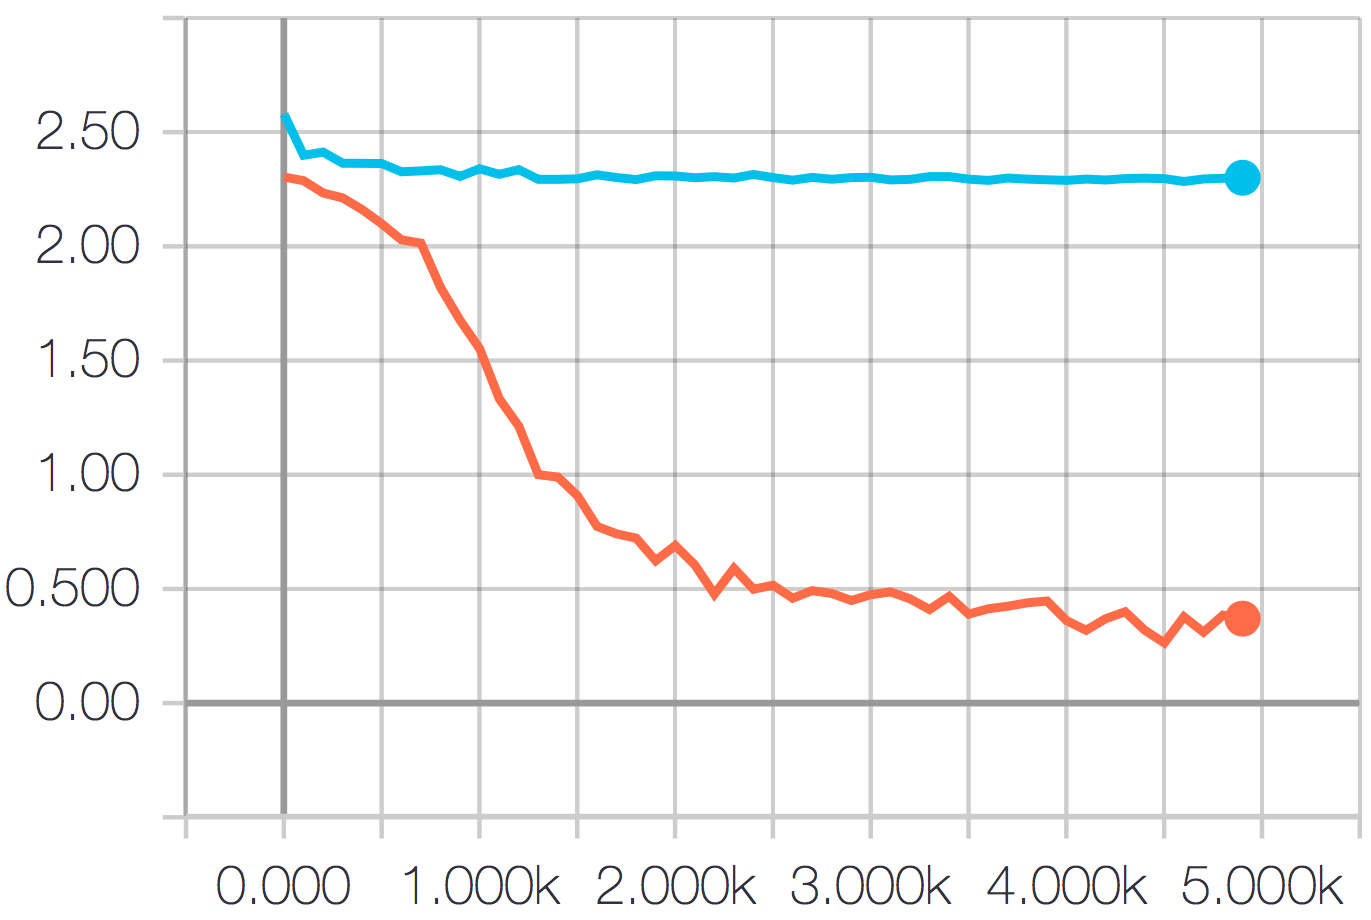
\includegraphics[width=8cm]{images/af_loss.png} % requires the graphicx package
   \caption{The figure shows the loss training data of {\tt ReLu} (orange) and {\tt Sigmoid} (cyan) activation function. }
   \label{fig:af_loss}
\end{figure}









\clearpage
\section{Adjust hyper-parameters: stage II}
\label{stage2}
In this chapter, we use the hyper-parameters optimzied in section \ref{stage1} and adjust the optimizer. There are three choices of optimizers: {\tt Gradient Descent} (base model), {\tt Adam Optimizer} and {\tt Momentum Optimizer}. We will explain more about later two optimizers.



\subsection{Adam optimizer}
Adaptive Moment Estimation (Adam) is a method that computes adaptive learning rates for each parameter. In addition to storing an exponentially decaying average of past squared gradients, Adam also keeps an exponentially decaying average of past gradients, similar to momentum.
Here we set the parameters of AdamOptimizer as: 

\begin{lstlisting}
optimizer = tf.train.AdamOptimizer(learning_rate=1E-1)
\end{lstlisting}


The plot of training loss is showed as Figure \ref{fig:adam}. Obviously the loss function is very high does not decrease at all.  As a matter of fact the accuracy rate is around 10\%.


\begin{figure}[!htb]
   \centering
   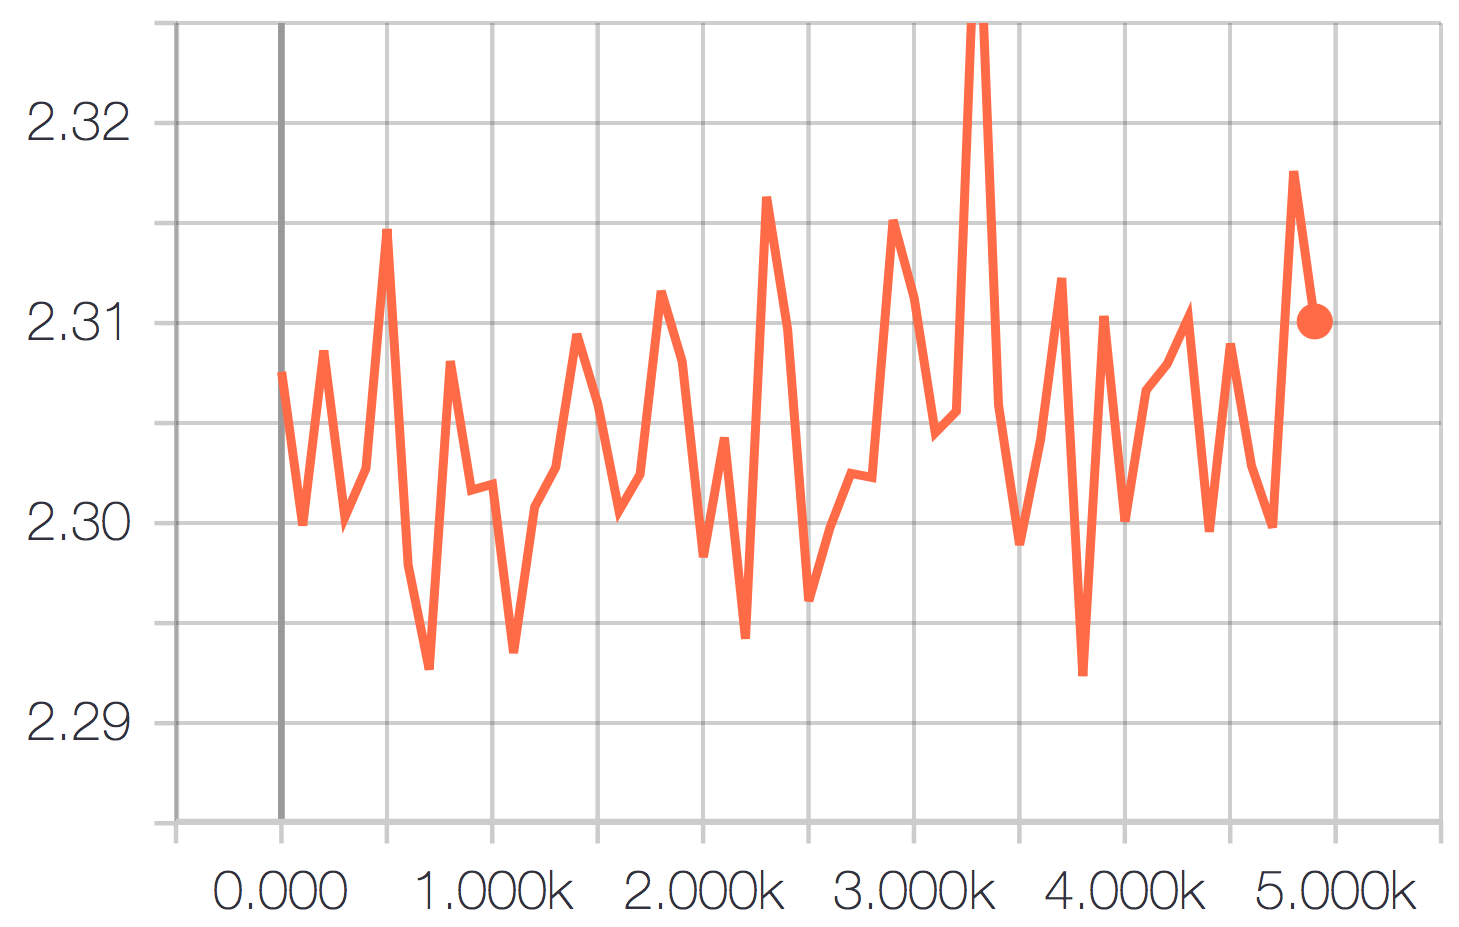
\includegraphics[width=10cm]{images/optimizer-adam.png} % requires the graphicx package
   \caption{Loss function of training data using Adam optimizer.}
   \label{fig:adam}
\end{figure}



\subsection{Momentum optimizer and SGD}
Steepest gradient descent (SGD) has trouble navigating ravines, i.e. areas where the surface curves much more steeply in one dimension than in another, which are common around local optima. Momentum is a method that helps accelerate SGD in the relevant direction and dampens oscillations. 

Here we set the parameters of MomentumOptimizer as: 

\begin{lstlisting}
optimizer = tf.train.MomentumOptimizer(learning_rate=1E-1, momentum=0.9)
\end{lstlisting}

The momentum is usually set to be 0.9.

The plot of training loss is showed as Figure \ref{fig:momentum-loss}. It seems both optimizers gives good result and oscillate starting at 2500 steps. In addition, the validation accuracy also shows the similar trend in Figure \ref{fig:momentum-accuracy}. Since the at the final step (5000 step) Momentum Optimizer has better accuracy (0.9891) then SGD (0.9881) and  Momentum Optimizer takes about 20\% less time to finish 5000 steps, it is reasonable to set Momentum Optimizer as our final optimizer.

\begin{figure}[!htb]
   \centering
   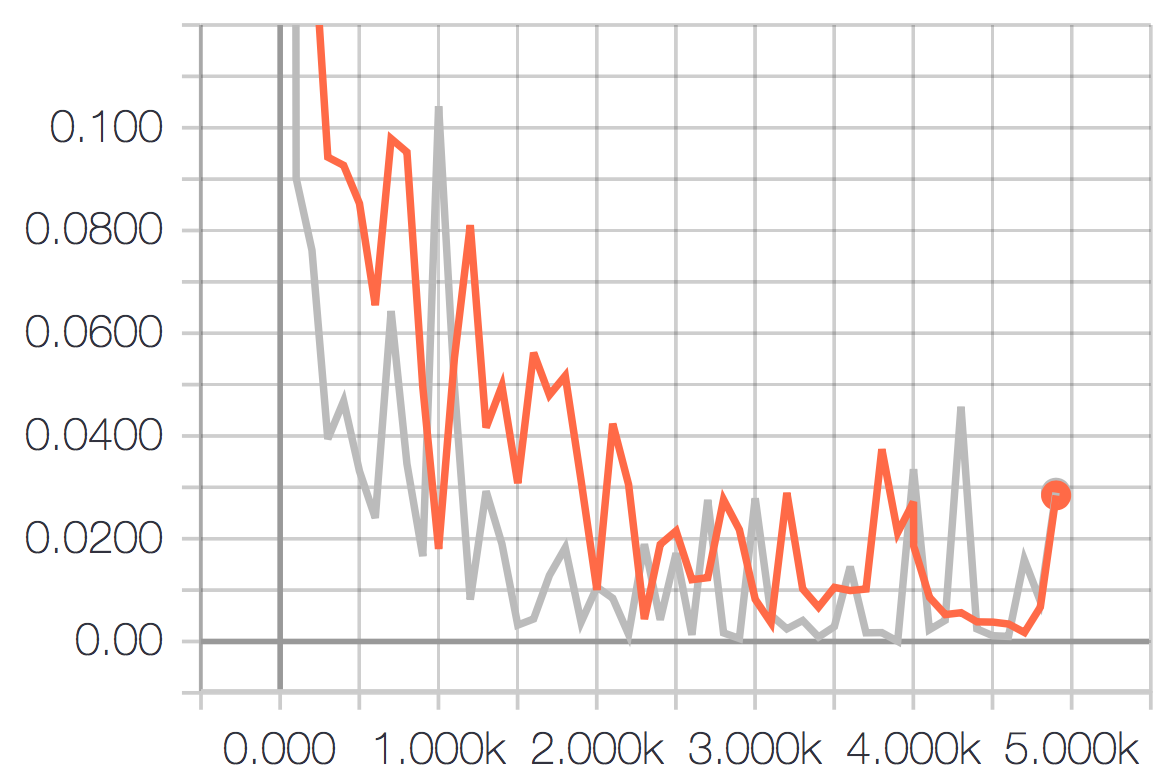
\includegraphics[width=10cm]{images/optimizer-loss.png} % requires the graphicx package
   \caption{Loss function of training data using Momentum Optimizer (grey) and SGD (orange).}
   \label{fig:momentum-loss}
\end{figure}


\begin{figure}[!htb]
   \centering
   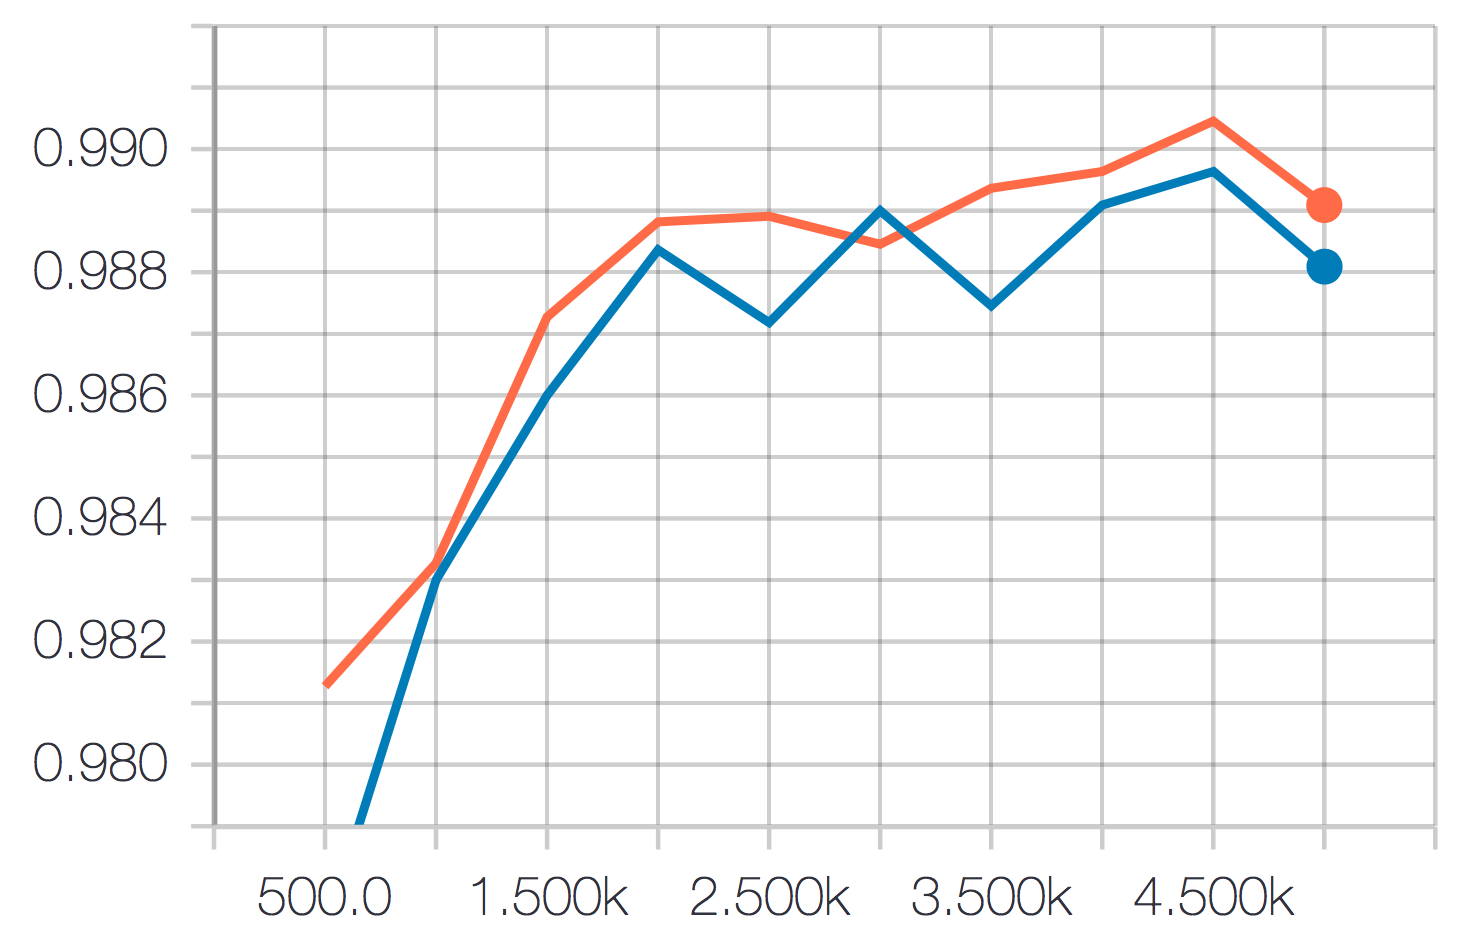
\includegraphics[width=10cm]{images/optimizer-accuracy.png} % requires the graphicx package
   \caption{Accuracy of validation data using Momentum Optimizer (orange) and SGD (blue).}
   \label{fig:momentum-accuracy}
\end{figure}

\clearpage

\section{Final model and analysis}
\label{summary}

Based on previous experiments, the final model contins the following hyper-parameters:

\begin{itemize}
\item
learning rate: {\tt 1E-1} 

\item
Size of filter:  $5\times5$

\item
Number of filters: 32 for first convolutional layer and 64 for second convolutional layer

\item
Number of convolutional and pooling layers: 2 and 2. The structure of the whole model is shown in Figure \ref{fig:2-c-2-p}.

\item
The ways of paddings: {\tt same}

\item
The choice of activation function: {\tt ReLu}

\item
Optimizer: {\tt Momentum Optimizer}
\end{itemize}
The source code containing these parameters is listed at the end of report. The loss of training process is presented in Figure \ref{fig:best-loss}. It shows the loss decrease dramatically at initial 100 steps and then tend to oscillate around a very low loss. Meanwhile, Figure \ref{fig:best-accuracy} shows the accuracy of validation data throughout the training process and it clearly shows the model accuracy increases and converge fast to a very hight value. The finally validation accuracy at step 5000 is 0.9891. With this model, the final testing accuracy is a very satisfactory which is 0.9910.


\begin{figure}[!htb]
   \centering
   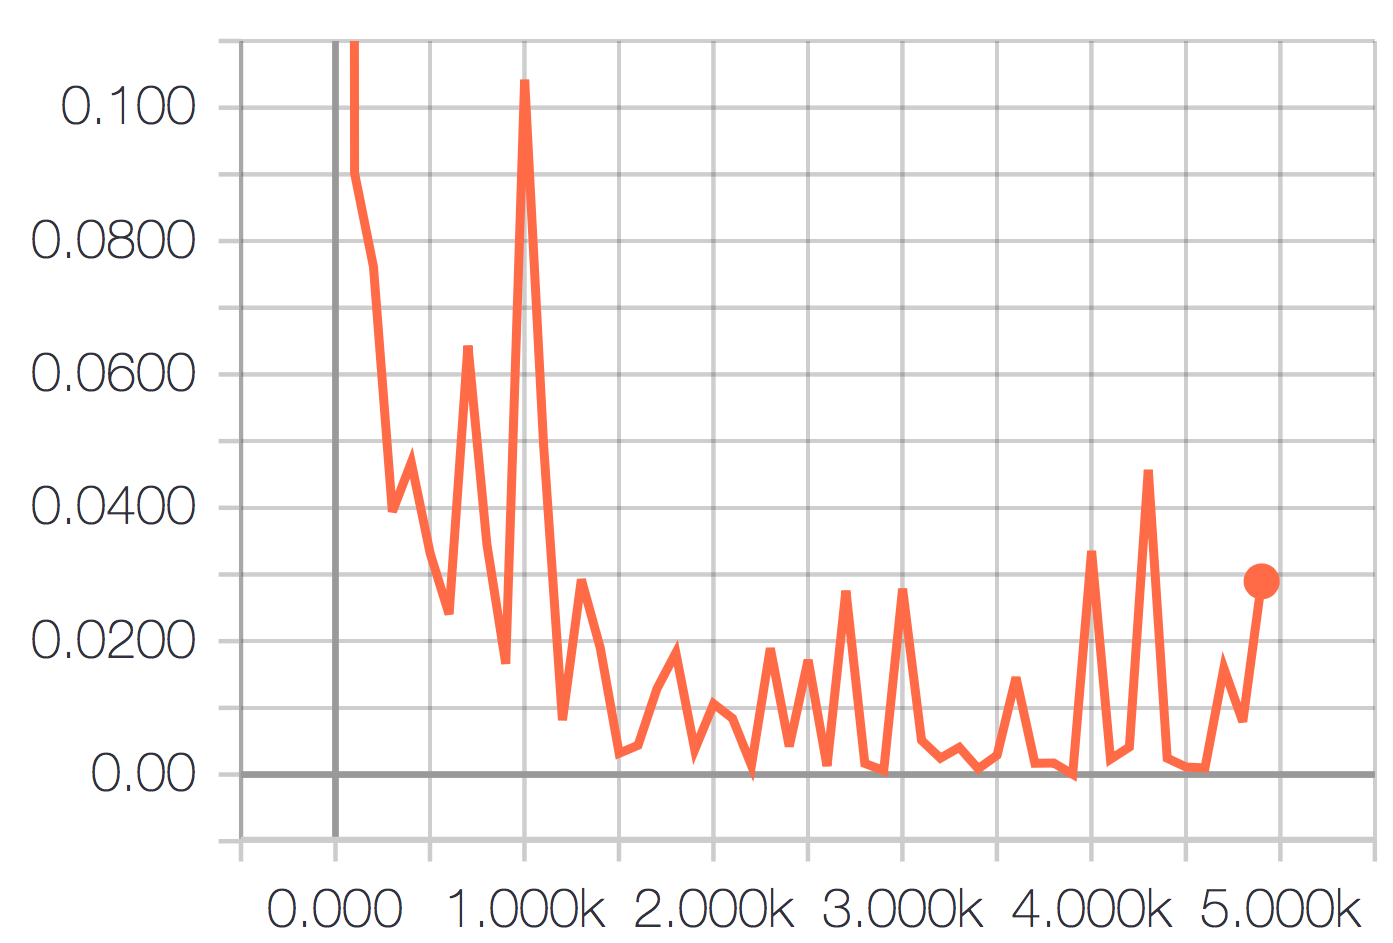
\includegraphics[width=10cm]{images/best_loss.png} % requires the graphicx package
   \caption{Loss of training.}
   \label{fig:best-loss}
\end{figure}




\begin{figure}[!htb]
   \centering
   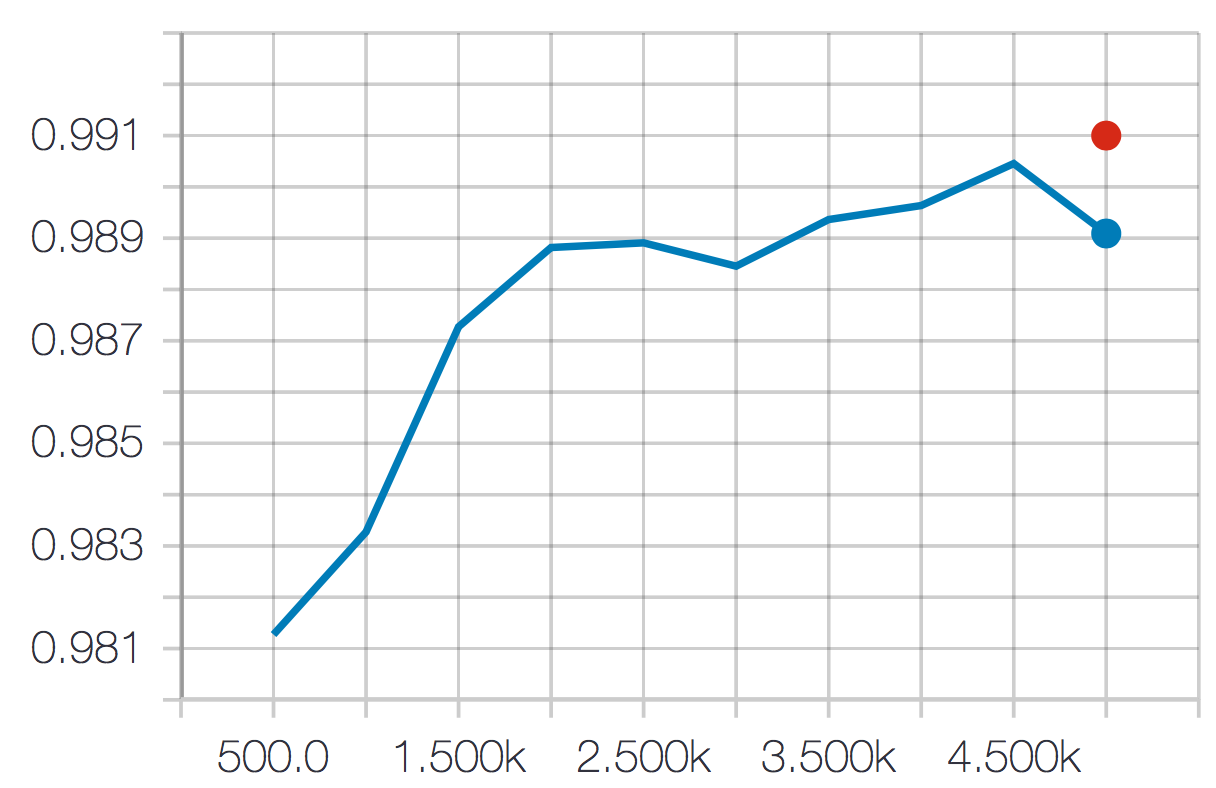
\includegraphics[width=10cm]{images/best_accuracy.png} % requires the graphicx package
   \caption{Accuracy of validation data (blue curve) and the final testing data (red dot).}
   \label{fig:best-accuracy}
\end{figure}






\clearpage
\section{Source codes}

Here we only present the source code that gives the best result.

\pythonexternal{./../best_model.py}




\vspace{24pt}



\end{document}


